\subsection{UC11 - Visualizzazione dei risultati della previsione}
\begin{figure}[H]
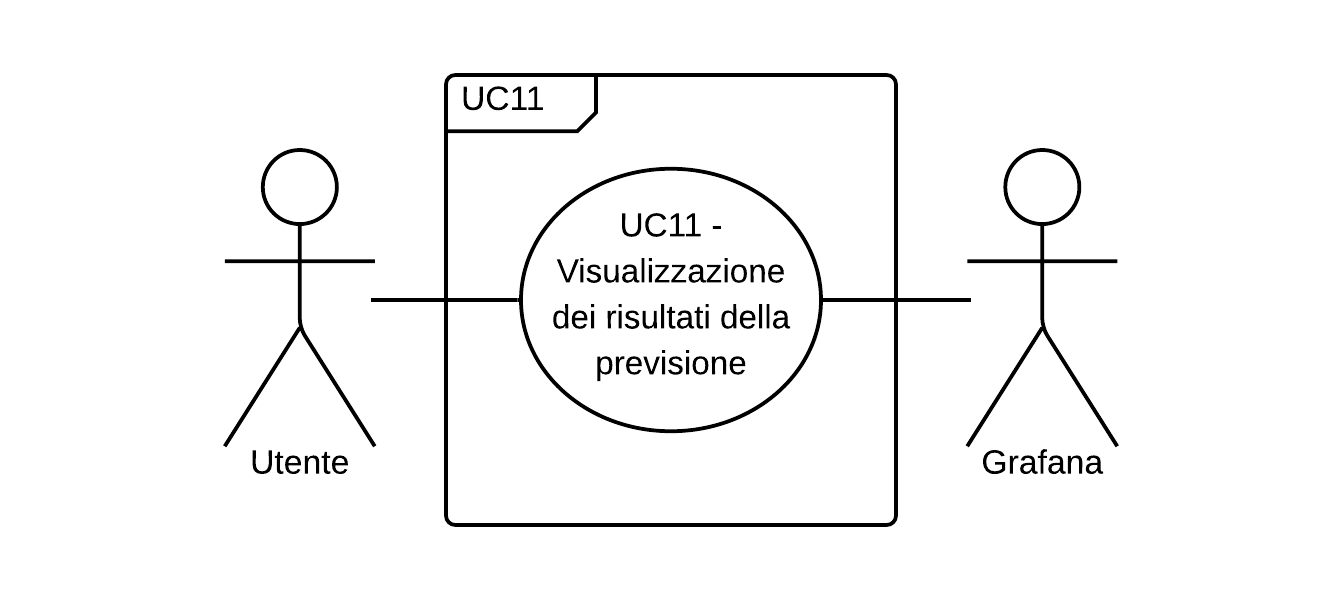
\includegraphics{img/UC11_-_Visualizzazione_dei_risultati_della_previsione.png}
\caption{Diagramma degli use case di UC11}
\end{figure}
\begin{itemize}
    \item \textbf{Codice identificativo}: UC11;
    \item \textbf{Titolo}: visualizzazione dei risultati della previsione;
    \item \textbf{Attori primari}: utente;
    \item \textbf{Attori secondari}: Grafana\glo;
    \item \textbf{Descrizione}: l'utente visualizza un grafico che riporta il risultato della previsione effettuata sul flusso dati;
    \item \textbf{Precondizioni}: l'utente è autenticato nel sistema software Grafana\glosp, ha avviato il plug-in, ha inserito il JSON per l'addestramento del modello e associato i nodi al flusso dati in maniera corretta;
    \item \textbf{Postcondizioni}: l'utente visualizza un grafico che riporta il risultato della previsione effettuata sul flusso dati;
    \item \textbf{Scenario principale}: l'utente visualizza un grafico che riporta il risultato della previsione effettuata sul flusso dati.
\end{itemize}